\documentclass[DIN, pagenumber=false, fontsize=11pt, parskip=half]{scrartcl}
\usepackage[UTF8]{ctex}  % 中文支持
% \usepackage{ngerman}
\usepackage[utf8]{inputenc}
\usepackage[T1]{fontenc}
\usepackage{textcomp}
\usepackage{graphicx}
\usepackage{amsmath}
\usepackage{booktabs}
\usepackage{tasks}
\usepackage{xcolor} % Required for custom red
\usepackage{amsmath,amssymb}
\usepackage{tikz}
\usetikzlibrary{calc}
\usepackage{geometry} % Custom margins

\usepackage{tocloft} % Modifying the table of contents

% for matlab code
% bw = blackwhite - optimized for print, otherwise source is colored
\usepackage[framed,numbered,bw]{mcode}
\usepackage[most]{tcolorbox}
% for other code
%\usepackage{listings}

\setlength{\parindent}{0em}

% set section in CM
\setkomafont{section}{\normalfont\bfseries\Large}

\newcommand{\mytitle}[1]{{\noindent\Large\textbf{#1}}}
\newcommand{\mysection}[1]{\textbf{\section*{#1}}}
\newcommand{\mysubsection}[2]{\romannumeral #1) #2}

\newtcolorbox{parchmentquote}{
    enhanced,
    colback=orange!5!white,   % 浅米黄色背景
    colframe=orange!50!black,
    boxrule=0.5pt,
    arc=2pt,                  % 细微圆角
    boxsep=5pt,
    before skip=10pt,
    after skip=10pt,
    fontupper=\itshape,
    borderline west={2pt}{0pt}{orange!80!black} % 加厚的左装饰线
}
%===================================
\begin{document}
\newcommand{\blank}[1][3em]{\underline{\hspace{#1}}}
\noindent\textbf{课后练习} \hfill \textbf{online course}\\
primary school \hfill Liu\\

\mytitle{分数练习 \hfill \today}
\newline
\begin{parchmentquote}
    本节课主要复习分数的性质。
    从基础开始，分数与小数的转换，分数加减尤其异分母加减。


\end{parchmentquote}

\begin{enumerate}
  \item 截至2025年3月，我国高速铁路运营里程已达到 $48000000$ 米，横线上的数读作：\blank[6em]；
  其中某条重要干线累计运送旅客超 $12896500$ 人次，用“四舍五入”法省略万后面的尾数约是 \blank[4em] 万人。

  \item $35\%=14:\blank[4em]=\blank[4em]\div 60=\blank[4em]\text{折}-\dfrac{\blank[2em]}{\blank[2em]}\ (\text{最简分数})$

  \item $a$ 和 $b$ 为不同的质数（$a<b$），且
  $\dfrac{1}{a}+\dfrac{1}{b}=\dfrac{10}{21}$，
  则 $a=\blank[3em]$，$b=\blank[3em]$。

  \item 某机场新开通一条航线，在比例尺为 $1:8000000$ 的地图上，图上 $1$ 厘米表示实际是 \blank[3em] 千米；
  量得该航线长度为 $18$ 厘米，实际航程为 \blank[3em] 千米。

  \item 杭州推行新能源汽车，每充一度电需花费 $1.2$ 元。
  明明爸爸的新能源汽车充满需 $60$ 度电，能续航 $400$ 千米，
  那每千米行驶成本为 \blank[3em] 元。
  明明爸爸从家到单位往返一次为 $70$ 千米，充满一次电后，最多往返 \blank[3em] 次。

  \item 明明养了一只鹦鹉，重约 $50$ \blank[2em]，
  鸟笼重约 $3$ 千克 $20$ 克，即重 \blank[3em] 千克。

  \item 欣欣果园里的桔子树丰收了，共收获 $1210$ 千克桔子，
  每 $20$ 千克装一箱，需要 \blank[3em] 个箱子才能装完；
  如果用 $3$ 千克的礼盒装，能装满 \blank[3em] 盒。

  \item 有 $2$ 个自然数 $m$ 和 $n$，其中 $m=3\times5\times7$，$n=2\times5\times3$，
  $m$ 和 $n$ 的最大公因数是 \blank[4em]，最小公倍数是 \blank[4em]。

  \item 如图，把一个半径是 $3\text{ dm}$ 的圆柱切开，拼成一个近似的长方体，
  表面积增加了 $72\text{ dm}^2$。这个圆柱的底面积是 \blank[4em] $\text{dm}^2$，
  圆柱的高是 \blank[4em] $\text{dm}$。

  \begin{center}
  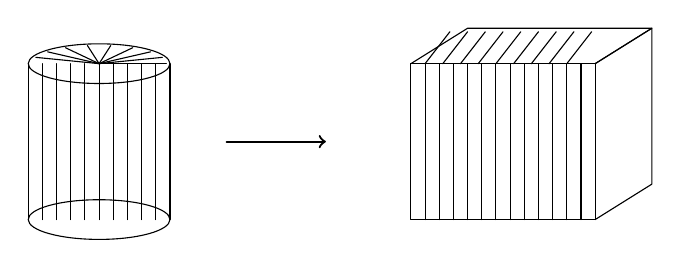
\begin{tikzpicture}[scale=0.9, line cap=round, line join=round]
    % --- cylinder ---
    \begin{scope}
      \draw (0,0) ellipse (1.0 and 0.28);
      \draw (-1,0)--(-1,-2.2);
      \draw ( 1,0)--( 1,-2.2);
      \draw (0,-2.2) ellipse (1.0 and 0.28);
      % vertical ribs
      \foreach \x in {-0.8,-0.6,...,0.8}{
        \draw (\x,0)--(\x,-2.2);
      }
      % top spokes
      \foreach \ang in {0,20,...,160}{
        \draw (0,0)--({0.95*cos(\ang)},{0.26*sin(\ang)});
      }
    \end{scope}

    % arrow
    \draw[->, thick] (1.8,-1.1)--(3.2,-1.1);

    % --- rectangular prism (approx.) ---
    \begin{scope}[xshift=4.4cm]
      \coordinate (A) at (0,0);
      \coordinate (B) at (2.6,0);
      \coordinate (C) at (2.6,-2.2);
      \coordinate (D) at (0,-2.2);
      \coordinate (E) at (0.8,0.5);
      \coordinate (F) at (3.4,0.5);
      \coordinate (G) at (3.4,-1.7);
      \coordinate (H) at (2.6,-2.2);

      \draw (A)--(B)--(C)--(D)--cycle;      % front face
      \draw (A)--(E)--(F)--(B);            % top face
      \draw (B)--(F)--(G)--(C);            % right face

      % front ribs
      \foreach \x in {0.2,0.4,...,2.4}{
        \draw (\x,0)--(\x,-2.2);
      }
      % top slanted marks
      \foreach \t in {0.2,0.45,...,2.35}{
        \draw (\t,0)--(\t+0.35,0.45);
      }
    \end{scope}
  \end{tikzpicture}
  \end{center}

 

\end{enumerate}

\end{document}